%\chapter{具体线路的复杂度与误差分析}

\chapter{含噪的变分量子线路模拟}\label{chap:noisy_vqa}

\section{背景介绍}
在如今NISQ时代,噪声难以避免的出现在量子线路中。这些噪声导致许多需要高保真度的量子算法难以实现。比如Shor算法需要使用到深层量子线路,因此对噪声的容忍度较低,在现有超导量子处理器上(单比特门错误率$\~10^{-3}$,两比特门$\~10^{-2}$)保真度将指数衰减至可忽略水平,导致计算失效。

为了在近期的量子设备中实现实用性的量子算法,变分量子算法(Variational Quantum Algorithm,VQA)~\cite{Cerezo2021variational,mcclean2016theory,tilly2022variational}作为最受欢迎的一类NISQ算法,普遍被认为是一个很好的解决方案。
变分量子算法通过将量子电路的参数优化与经典优化器相结合,其核心思想基于变分原理:构造变分量子线路,以产生作为试探的量子态,通过经典优化器调整参数,使系统能量或目标函数达到极值。
通过这一"量子执行-经典反馈"的混合结构,变分量子算法展示出独特的噪声适应性:仅仅依靠浅层量子线路(通常$<100$层)因此能够将噪声的积累限制在可以控制的范围内。

基于变分量子算法发展的一系列算法,已经在各个领域产生了广泛的应用:
在组合优化领域,量子近似优化算法~\cite{farhi2014quantum,moll2018quantum}(Quantum Approximate Optimization Algorithm,QAOA)通过将目标优化问题编码为物理系统的基态求解问题,通过交替应用混合哈密顿量和问题哈密顿量的演化来逼近基态能量。
在量子化学领域,变分量子本征求解器~\cite{peruzzo2014variational, kandala2017hardwarea,li2022toward}(Variational Quantum Eigensolver,VQE)通过变分量子线路模拟分子哈密顿量的基态能量,从而实现分子结构的计算。
在量子机器学习领域,量子支持向量机~\cite{havlivcek2019supervised}(Quantum Support Vector Machine,QSVM)通过变分量子线路实现量子数据的分类,以及量子神经网络~\cite{beer2020training,huang2021experimental, mitarai2018quantum}(Quantum Neural Network,QNN)通过变分量子线路实现量子数据的学习。
在量子纠错领域,基于变分的量子纠错~\cite{johnson2017qvector,xu2021variational}通过变分量子线路实现量子纠错码的编码和解码。


虽然变分量子算法作为NISQ时代最有希望的候选者,并且已经开发了一系列的应用,但是在实际应用中,是否能在NISQ设备中利用变分量子算法产生实际的量子优势仍然是一个开放的问题。其中一个主要的挑战是变分量子算法的鲁棒性:在NISQ设备中,由于噪声的存在,变分量子算法的性能会受到严重影响。为了研究噪声下变分量子算法的优势,我们将通过OBPPP算法对其进行模拟,研究其产生量子优势的条件。


在本节的讨论中,我们将变分量子线路的深度记为 $L$,即 $\mathcal{U}(\bm{\theta})=\mathcal{U}_L(\bm{\theta}_L)\cdots\mathcal{U}_1(\bm{\theta}_1)$。变分量子线路的每一层 $\mathcal{U}_i(\bm{\theta}_i)$ 是由 $R_i$ 个旋转门和 $C_i$ 个 Clifford 门组成,这些门作用于相互不相交的量子比特上,$\bm{\theta}_i=(\theta_{i,1},\cdots,\theta_{i,R_i})$ 表示第 $i$ 层的参数向量,$\bm{\theta}=(\bm{\theta}_1,\cdots,\bm{\theta}_L)$ 表示整个变分量子线路的参数向量。
具体来说,第 $i$ 层中的第 $j$ 个旋转门表示为 $U_{i, j}(\theta_{i,j})=\exp{-i \frac{\theta_{i,j}}{2} \sigma_{i,j}}$,其中 $j \in \{1, \cdots , R_i\}$,$\theta_{i,j}$ 是旋转角度,$\sigma_{i, j}\in \{\mathbb{I}, X,Y,Z\}^{\otimes n}$为Pauli旋转门对应的Pauli算符。
类似地,第 $i$ 层中的第 $k$ 个 Clifford 门表示为 $V_{i,k}$,其中 $k \in \{1, \cdots , C_i\}$。$V_{i,k}\in\{\mathrm{H}(a),\mathrm{S}(a),\mathrm{CNOT}(a,b)\}$,其中 $a,b $ 指的是门作用的量子比特的序号。

记所有Pauli旋转门 $U_{i,j}(\theta_{i,j})$ 的 Pauli 算符集合为 $\{\sigma_{i,j}\}$。
我们将集合 $\{\overline{\sigma}_{i,j}\}$ 表示为经过后续 Clifford 门变换后的所有 $\sigma_{i,j}$,即 $\overline{\sigma}_{i,j}= \mathcal{V}_{L} \cdots \mathcal{V}_{i} \sigma_{i,j} \mathcal{V}_{i}^\dagger \cdots \mathcal{V}_{L}^\dagger$,其中 $\mathcal{V}_{i} = \prod_{k=1}^{C_i} V_{i,k}$ 是对应于第 $i$ 层中所有 Clifford 门的张量积的幺正变换。

为了确保引理~\ref{lemma:cross_items} 的有效性,我们需要一个容易实现的前提条件:假设集合 $\{\overline{\sigma}_{i,j}\}$ 在忽略相位的意义下,可以生成 $\{\mathbb{I}, X, Y, Z\}^{\otimes n}$。这一条件可以通过以下等式来表示:
\begin{equation}\label{eq:generate}
  \langle \{\overline{\sigma}_{i,j}\}\rangle/\left(\langle \{\overline{\sigma}_{i,j}\}\rangle\cap\langle i\mathbb{I}^{\otimes n}\rangle\right)=\{\mathbb{I},X,Y,Z\}^{\otimes n},
\end{equation}
这里 $\langle \{\overline{\sigma}_{i,j}\} \rangle$ 指的是由集合 $\{\overline{\sigma}_{i,j}\}$ 生成的 Pauli 子群,这意味着 $\langle \{\overline{\sigma}_{i,j}\}\rangle$ 中的元素可以表示为 $\{\overline{\sigma}_{i,j}\}$ 中元素的有限乘积。
为了证明这一条件确实容易满足,考虑在电路的最后两层中,每个量子比特上都有一层 $R_X$ 门和一层 $R_Z$ 门作用,那么 $\{X_i, Z_i\}_{i=1,\cdots,n}$ 包含在 $\{\overline{\sigma}_{i,j}\}$ 中。这些 $\{ X_i,Z_i \}_{i=1,\cdots,n}$ 足以生成 $\{\mathbb{I},X,Y,Z\}^{\otimes n}$。事实上,这一充分条件可以进一步减弱,如第~\ref{temp:subsubsection:cross_items}节 中所示。


\section{计算复杂度分析}

在本节中,我们将估计使用OBPPP算法模拟含噪声变分量子线路的计算复杂度。根据式~\eqref{eq:total_cost}我们可以看到,计算$\widehat{\langle O \rangle}$的时间复杂度可以表示为$C = C_s+N_MC_f$,其中$C_s$是枚举所有满足条件的Pauli路径的时间复杂度,$N_M$是满足条件的Pauli路径的数量,$C_f$是计算每个Pauli路径的贡献的时间复杂度。
其中$C_f$可以进一步分解为$C_{f\mathcal{U}}+C_{fO}+C_{f\rho}$,其中$C_{f\mathcal{U}}$是计算与中间量子门关联的项$\prod\Tr{s_i\mathcal{U}_i s_{i-1}\mathcal{U}_i^\dagger}$的时间复杂度,$C_{fO}$是和观测量相关的$\Tr{Os_L}$项的时间复杂度,$C_{f\rho}$是和初态相关的$\Tr{\rho s_0}$项的时间复杂度。

对于空间复杂度,根据式~\eqref{eq:space_cost},我们可以得到$S = S_s+S_f$,其中$S_s$是枚举所有满足条件的Pauli路径的空间复杂度,$S_f$是计算每个Pauli路径的贡献函数的空间复杂度。根据式~\eqref{eq:space_f},$S_f$可以进一步分解为$\max\{S_{f\mathcal{U}},S_{fO},S_{f\rho}\}$,其中$S_{f\mathcal{U}}$是计算与中间量子门关联的项$\prod\Tr{s_i\mathcal{U}_i s_{i-1}\mathcal{U}_i^\dagger}$的空间复杂度,$S_{fO}$是和观测量相关的$\Tr{Os_L}$项的空间复杂度,$S_{f\rho}$是和初态相关的$\Tr{\rho s_0}$项的空间复杂度。

在第~\ref{sec:obppp}节中,我们已经讨论了枚举所有满足条件的Pauli路径的时间复杂度$C_s$和空间复杂度$S_s$,以及在设定稀疏性条件下$C_{fO}$、$C_{f\rho}$和$S_{fO}$、$S_{f\rho}$的估计。
在本节中,我们将讨论对于变分量子线路$C_{f\mathcal{U}}$和$S_{f\mathcal{U}}$的估计,以及式~\eqref{eq:case1:cost_s}\eqref{eq:case1:N_M}\eqref{eq:case2:cost_s}\eqref{eq:case2:N_M}\eqref{eq:path:space_cost}中关联的$N_{\text{max}}$、$C_{\text{split}}$和$S_{\text{split}}$的估计。


为了估计$C_{f\mathcal{U}}$和$S_{f\mathcal{U}}$我们首先介绍以下命题:
\begin{proposition}\label{prop:layer_terms}
    计算 $f$ 中第 $i$ 层项的时间和空间复杂度为 $\order{n}$,可通过如下等式计算:
    \begin{equation}\label{eq:i-layer_terms}
    \begin{aligned}
    \Tr{s_i\mathcal{U}_i s_{i-1}\mathcal{U}_i^\dagger}&=\Tr{\left(s_i s_{i-1}\right)\big|_{I_i}}\\
    \prod_{k=1}^{C_i}&\Tr{\left(s_iV_{i,k} s_{i-1}V_{i,k}^{\dagger}\right)\big|_\g{V_{i,k}}}\prod_{\sigma_{i,j}\in C(i,s_{i-1})}\Tr{\left(s_i s_{i-1}\right)\big|_\g{\sigma_{i,j}}}\\
    \prod_{\sigma_{i,j'}\in AC(i,s_{i-1})} &\Bigg\{ \Tr{\left(s_i s_{i-1}\right)\big|_\g{\sigma_{i,j'}}}\cos{\theta_{i,j'}}- \Tr{\left(is_i \sigma_{i,j'}s_{i-1}\right)\big|_\g{\sigma_{i,j'}}}\sin{\theta_{i,j'}}  \Bigg\},
    \end{aligned}
    \end{equation}
    其中$\supp:\{\mathbb{I}, X, Y, Z\}^{\otimes n}\cup\{\mathrm{CNOT}_{a,b},\mathrm{H}_a,\mathrm{S}_a\}\rightarrow2^{\{1,\cdots, n\}}$ 为从幺正算符到其非平凡作用的量子比特的映射。这里 $2^{\{1,\cdots, n\}}$ 表示 $\{1,\cdots, n\}$ 的所有子集。
    为了简化,我们将 $i$ 层中 $n$ 个量子比特的索引根据所应用门的类型分为三组。这些组分别表示为符号 $\big|_{I_i}$、$\big|_\g{V_{i,k}}$ 和 $\big|_\g{\sigma_{i,j}}$,对应于没有门作用、Clifford 门作用和 Pauli 旋转门作用。此外,集合 $C(i,s_{i-1})$ 和 $AC(i,s_{i-1})$ 分别表示 $\{\sigma_{i,j}\}_{j=1}^{R_i}$ 中与 $s_{i-1}$ 对易和反对易的 Pauli 算符集合。
    
    \begin{proof}
    
    在变分量子线路中,$\mathcal{U}_i$ 由一系列门 $U_{i,1},\cdots,U_{i,R_i}$ 和 $V_{i,1},\cdots,V_{i,C_i}$ 组成,并且不会在每个量子比特上操作两次。
    Pauli 旋转门 $U_{i,j}(\theta_{i,j})$ 的形式为:
    \begin{equation}
      U_{i,j}(\theta_{i,j})=\exp{-i \frac{\theta_{i,j}}{2} \sigma_{i,j}}.
    \end{equation}
    
    Clifford 门 $V_{i,k}$ 可以从 $\{\mathrm{H}(a),\mathrm{S}(a),\mathrm{CNOT}(a,b) \}_ {a\neq b}$ 中选择。
    因此,我们有:
    \begin{equation}
      \begin{aligned}
        \Tr{s_i\mathcal{U}_i s_{i-1}\mathcal{U}_i^\dagger}=&\Tr{\left(s_i s_{i-1}\right)\big|_{I_i}}
        \prod_{k=1}^{C_i}\Tr{\left(s_iV_{i,k} s_{i-1}V_{i,k}^{\dagger}\right)\big|_\g{V_{i,k}}}\\
        &\prod_{j=1}^{R_i}\Tr{\left(s_i U_{i,j}(\theta_{i,j}) s_{i-1} U_{i,j}^\dagger(\theta_{i,j})\right) \big|_\g{\sigma_{i,j}}}.
      \end{aligned}
    \end{equation}
    
    厄米 算符 $X$ 的指数定义为 $\exp{X}=\sum_{k=0}^\infty\frac{X^k}{k!}$。对于 Pauli 算符,任何 Pauli 算符号的满足自反性 $\sigma^2=\mathbb{I}$,因此我们有:
    \begin{equation}
      \exp{-i \frac{\theta}{2} \sigma}=\sum_{k=0}^\infty\frac{(-i \frac{\theta}{2}\sigma)^k}{k!}=\sum_{k=0}^\infty\frac{(-1)^k (\frac{\theta}{2})^{2k}}{(2k)!} \mathbb{I}- i\frac{(-1)^k (\frac{\theta}{2})^{2k+1}}{(2k+1)!}\sigma=\cos{\frac{\theta}{2}}\mathbb{I}-i \sin{\frac{\theta}{2}}\sigma.
    \end{equation}
    
    根据 Pauli算符$\sigma$ 和另一个 Pauli算符 $\sigma'$ 的对易/反对易关系,有:
    \begin{equation}
    \begin{aligned}
    &\sigma'\exp{-i \frac{\theta}{2} \sigma}=\exp{-i \frac{\theta}{2} \sigma}\sigma',\text{ 如果 }\sigma\text{ 与 }\sigma'\text{ 对易。}\\
    &\sigma'\exp{-i \frac{\theta}{2} \sigma}=\exp{i \frac{\theta}{2} \sigma}\sigma',\text{ 如果 }\sigma\text{ 与 }\sigma'\text{ 反对易。}\\
    \end{aligned}
    \end{equation}
    因此可以将 $\{\sigma_{i,j}\}$ 分为两种情况。如果 $\sigma_{i,j}$ 与 $s_{i-1}$ 对易,有:
    
    \begin{equation}
      \begin{aligned}
      \Tr{\left(s_i U_{i,j}(\theta_{i,j}) s_{i-1} U_{i,j}^\dagger(\theta_{i,j})\right)\big|_\g{\sigma_{i,j}}}
      &=\Tr{(s_i \exp{-i \frac{\theta_{i,j}}{2}\sigma_{i,j} }  \exp{i \frac{\theta_{i,j}}{2}\sigma_{i,j} }s_{i-1}) \big|_\g{\sigma_{i,j}}}\\
      &=\Tr{(s_i \exp{-i \frac{\theta_{i,j}}{2}\sigma_{i,j} } \exp{i \frac{\theta_{i,j}}{2}\sigma_{i,j} }s_{i-1}) \big|_{\g{\sigma_{i,j}}}}\\
      &=\Tr{(s_i s_{i-1})\big|_{\g{\sigma_{i,j}}}}.
    \end{aligned}
    \end{equation}
    而若 $\sigma_{i,j}$ 与 $s_{i-1}$ 反对易,则有:
    \begin{equation}
      \begin{aligned}
      &\Tr{\left(s_i U_{i,j}(\theta_{i,j}) s_{i-1} U_{i,j}^\dagger(\theta_{i,j})\right)\big|_\g{\sigma_{i,j}}}\\
      &=\Tr{ \left(s_i\exp{-i \frac{\theta_{i,j}}{2}\sigma_{i,j} } s_{i-1}\exp{i \frac{\theta_{i,j}}{2}\sigma_{i,j}}\right) \big|_\g{\sigma_{i,j}}}\\
      &=\Tr{\left( s_i  \exp{-i\theta_{i,j}\sigma_{i,j}} s_{i-1}\right) \big|_\g{\sigma_{i,j}}}\\
      &=\Tr{ \left(s_i (\cos{\theta_{i,j}}\mathbb{I}-i\sin{\theta_{i,j}}\sigma_{i,j}) s_{i-1} \right) \big|_\g{\sigma_{i,j}}}\\
      &=\Tr{\left(s_i s_{i-1}\right)\big|_\g{\sigma_{i,j}}}\cos{\theta_{i,j}}-\Tr{\left(i s_i \sigma_{i,j}s_{i-1}\right)\big|_\g{\sigma_{i,j}}}\sin{\theta_{i,j}}.
    \end{aligned}
    \end{equation}
    以上完成了 式.~\eqref{eq:i-layer_terms} 的证明。

    此外,对于计算复杂度,可以分类讨论。
    对$\big|_{I_i}$项,需要比较$s_i$ 和 $s_{i-1}$ 在$\supp(I_i)$上是否相同。这一操作的时间和空间复杂度为 $\order{n}$。
    对于$\big|_\g{V_{i,k}}$项,需要比较$s_i$ 和 $V_{i,k}s_{i-1}V_{i,k}^\dagger$ 在$\supp(V_{i,k})$上是否相同,因为 $V_{i,k}\in\{\mathrm{H}(a),\mathrm{S}(a),\mathrm{CNOT}(a,b)\}$,$V_{i,k}s_{i-1}V_{i,k}^\dagger$ 可以在 $\order{1}$ 的时间内计算。因此,对于所有$\big|_\g{V_{i,k}}$项,总的时间和空间复杂度为 $\order{n}$。
    对于$\big|_\g{\sigma_{i,j}}$项,需要首先比较$s_{i-1}$ 和 $\sigma_{i,j}$ 在$\supp(\sigma_{i,j})$上的对易关系,然后再比较$s_i$ 和 $s_{i-1}$(或是$\sigma_{i,j'}s_{i-1}$) 在$\supp(\sigma_{i,j})$上是否相同。这两个操作的时间和空间复杂度为均为 $\order{\abs{\supp(\sigma_{i,j})}}$。因此,对于所有$\big|_\g{\sigma_{i,j}}$项,总的时间和空间复杂度为 $\order{n}$。

    综上所述,计算 $f$ 中第 $i$ 层项的时间和空间复杂度为 $\order{n}$。
    \end{proof}
\end{proposition}

\begin{remark}\label{remark:f_ele}
通过利用不同 Pauli 算符的正交性,可以在 $\Tr{s_i\mathcal{U}_i s_{i-1}\mathcal{U}_i^\dagger} \neq 0$ 时,建立以下$s_i$ 和 $s_{i-1}$ 之间的关系:

\begin{tabular}{|c|c|c|}
  \hline
   项 & 关系 & $f$ 中的因子\\
  \hline
  ${I_i}$ &$s_{i-1}\big|_{I_i} = s_{i}\big|_{I_i}$& 1 \\
  \hline
  $V_{i,k}$ &$s_{i-1}\big|_\g{V_{i,k}}= \pm V_{i,k}^{\dagger} s_{i}V_{i,k}\big|_\g{V_{i,k}}$& $\pm 1$ \\
  \hline
  $C(i,s_{i-1})=C(i,s_{i})$&$s_{i}|_\g{\sigma_{i,j}}=s_{i-1}|_\g{\sigma_{i,j}}$& 1 \\
  \hline
  \multirow{2}{*}{$AC(i,s_{i-1})=AC(i,s_{i})$}
  &$s_{i}|_\g{\sigma_{i,j}}=s_{i-1}|_\g{\sigma_{i,j}}$& $\cos{\theta_{i,j}}$ \\
  \cline{2-3}
  &$s_{i}|_\g{\sigma_{i,j}}=\pm i \sigma_{i,j} s_{i-1}|_\g{\sigma_{i,j}}$& $\mp \sin{\theta_{i,j}}$ \\
  \hline
\end{tabular}

以上表格中的关系可以帮助我们计算 $f$ 中的每一项。以$I_i$ 为例,该表格表面若$\bm{s}$有非平凡贡献$f(\mathcal{U},\bm{s},O,\rho) \neq 0$,则必有$s_{i-1}\big|_{I_i} = s_{i}\big|_{I_i}$。这意味着 $s_{i-1}$ 和 $s_{i}$ 在第 $i$ 层的第 $j$ 个旋转门上的作用是相同的。且这一关系为$f$带来了一个因子1。

通过命题~\ref{prop:layer_terms},可以得知对于变分量子线路中的每一层,计算 $f$ 中的每一项的时间和空间复杂度为 $\order{n}$。因此,计算 $f$ 中的所有项的时间复杂度为 $\order{L n}$,得到式~\eqref{eq:cost_f}中$C_{f\mathcal{U}}=\order{L n}$。式~\eqref{eq:space_f}中的$S_{f\mathcal{U}}=\order{n}$。
\end{remark}

结合式~\eqref{eq:cost_rho}和式~\eqref{eq:cost_O},我们可以得到式~\eqref{eq:cost_f}对于变分量子线路取值为:
\begin{equation}\label{eq:vqa:c_f}
    C_f=\order{L n}+\order{n}+\order{\poly(n)}=\order{\poly(n)+L n}.
\end{equation}
式~\eqref{eq:space_f}对于变分量子线路取值为:
\begin{equation}
    S_f=\max\{\order{n},\order{\poly(n)},\order{\poly(n)}\}=\order{\poly(n)}.
\end{equation}


在OBPPP算法的复杂度的分析中,还涉及到对一个给定的Pauli算符$s$和构成线路$\mathcal{U}$的门集合$\{U_{i,j}\}$,求解以下集合:
\begin{equation}
    \left\{ s'\mid \Tr{s' U^\dagger_{i,j}s U_{i,j}}\neq 0 \right\}.
\end{equation}
为了估计整个算法的时间复杂度,我们需要考虑这一集合的最大元素数$N_{\text{max}}$、求解该集合所需要的时间$C_{\text{split}}$和空间复杂度$S_{\text{split}}$。

对于在变分线路中,每个门可最大分裂的Pauli 算符数量$N_{\max}$:
\begin{equation}
    N_{\text{max}} = \max_{i,j,s}\abs{ \left\{ s'\mid \Tr{s' U^\dagger_{i,j}s U_{i,j}}\neq 0 \right\}}.
\end{equation}
注意到,当 $U_{i,j}$ 为Clifford 门时,因为Clifford 门作用于Pauli 算符后仍为Pauli 算符,因此Clifford门不会增加Pauli 算符的数量。而当 $U_{i,j}$ 为Pauli 旋转门时,假设旋转的Pauli算符为$\sigma$。根据注释~\ref{remark:f_ele}当$s$与$\sigma$对易时,$s'=s$,因此最大分裂个数为1。当$s$与$\sigma$反对易时,$s'=s$ 或 $s'=\pm i \sigma s$,因此最大分裂个数为2。因此,$N_{\text{max}}=2$。

对于求解该集合所需要的时间$C_{\text{split}}$和空间复杂度$S_{\text{split}}$,对于Clifford门可以以$\order{1}$的时间和空间复杂度求解。对于Pauli 旋转门,需要比较$s$和$s'$的对易关系,并输出$s'$。这一操作的时间和空间复杂度为 $\order{n}$。因此,$C_{\text{split}}=\order{n}$,$S_{\text{split}}=\order{n}$。

因此,对于变分量子线路,对于\textbf{情况1}根据式~\eqref{eq:case1:N_M}和式~\eqref{eq:case1:cost_s},Pauli路径枚举过程的时间复杂度为:
\begin{equation}
    C_{s}=\mathrm{Poly}(n) \order{L} C_{\text{split}} N_{\text{max}}^{M}= \mathrm{Poly}(n) \order{L} 2^M.
\end{equation}
满足$\abs{\bm{s}}\leq M$的Pauli路径数量最多为:
\begin{equation}\label{eq:vqa:case1:N_M}
    N_M=\poly(n) N_{\text{max}}^{M}=\poly(n) 2^M.
\end{equation}

对于\textbf{情况2},根据式~\eqref{eq:case2:N_M}和式~\eqref{eq:case2:cost_s},Pauli路径枚举过程的时间复杂度为:
\begin{equation}
    C_{s}=\mathrm{Poly}(n) \order{(nL)^M} C_{\text{split}} N_{\text{max}}^{M}= \mathrm{Poly}(n) \order{(nL)^M} 2^M.
\end{equation}\label{eq:vqa:case2:N_M}
满足$\abs{\bm{s}}\leq M$的Pauli路径数量最多为:
\begin{equation}
    N_M=\poly(n)(nLN_{\text{max}})^{M+1}= \poly(n)(2nL)^{M+1}.
\end{equation}

对于枚举过程的空间复杂度,根据式~\eqref{eq:path:space_cost}:
\begin{equation}
    S_{s}=\order{\mathrm{Poly}(n)+\max\{S_{\text{split}},n\}L}=\order{\mathrm{Poly}(n)+nL}.
\end{equation}


综上所述,对于变分量子线路,根据式~\eqref{eq:total_cost}和式~\eqref{eq:space_cost},在给定截断参数$M$的情况下,含噪声期望值模拟的时间复杂度$C$和空间复杂度$S$分别为:
\begin{equation}\label{eq:vqa:cost}
    \begin{aligned}
        C&=\begin{cases}
            \mathrm{Poly}(n) \order{L} 2^M, & \text{如果$\abs{\bullet}_{\mathcal{N}}$属于\textbf{情况1}} \\
           \mathrm{Poly}(n) \order{(2nL)^{M+1}}, & \text{如果$\abs{\bullet}_{\mathcal{N}}$属于\textbf{情况2}}
        \end{cases}\\
        S&=\mathrm{Poly}(n)+nL,
    \end{aligned}
\end{equation}
其中$n$为量子比特数,$L$为线路深度,$\mathcal{N}$为噪声模型。


\section{误差分析}
在上一节中,已经得到了在给定截断参数$M$的情况下,模拟变分量子线路的计算复杂度(式~\eqref{eq:vqa:cost})。在这一节中,我们将讨论在给定的误差容忍度$\epsilon$下,如何选择截断参数$M$。

误差可以用均方误差(Mean Square Error, MSE)来衡量,对于一个随机变量$X$,其均方误差定义为$\mathbb{E}[(X-\hat{X})^2]$,其中$\hat{X}$是$X$的估计值。在这里,我们考虑的是含噪声期望值模拟的误差,即真实含噪声期望值$\widetilde{\langle O\rangle}$和其估计值$\widehat{\langle O\rangle}$之间的均方误差。根据定义(式~\eqref{eq:noise_expectation}和式~\eqref{eq:truncated_expectation}),含噪声期望值模拟的误差为:
\begin{equation}
    \widetilde{\langle O\rangle}-\widehat{\langle O\rangle}=\sum_{\abs{\bm{s}}_{\mathcal{N}}>M}f(\widetilde{\mathcal{U}},\bm{s},O,\rho),
\end{equation}
其中$\abs{\bullet}_{\mathcal{N}}$定义在式~\eqref{eq:noise_hamming_weight}中,表示与噪声模型$\mathcal{N}$关联的Hamming weight,$f(\widetilde{\mathcal{U}},\bm{s},O,\rho)$定义在式~\eqref{eq:noise_contribution}中,表示一个Pauli路径$\bm{s}$对含噪声期望值的贡献。


如果有式~\eqref{eq:generate}成立,有以下引理成立:
\begin{lemma}\label{lemma:cross_items}
    对于变分量子线路,如果式~\eqref{eq:generate}成立,则对任意两个不同的Pauli路径$\bm{s}$和$\bm{s}'$,有:
    \begin{equation}\label{eq:E_cross_equals_0}
        \mathbb{E}_{\bm{\theta}}\left[f(\widetilde{\mathcal{U}},\bm{s},O,\rho)f(\widetilde{\mathcal{U}},\bm{s}',O,\rho)\right]=0,
    \end{equation}
    其中期望是对于均匀随机选择的旋转角度$\bm{\theta}$。
\end{lemma}
我们先暂时跳过该引理的证明,我们将在后文中证明该引理。

关于均方误差,有以下引理:
\begin{lemma}\label{lemma:MSE_l}
    对于变分量子线路,如果式~\eqref{eq:E_cross_equals_0}成立,那么对任意的$\nu > 0$,只要截断参数$M$满足:
    \begin{equation}
        M\geq\frac{1}{4\gamma}\ln{\frac{\norm{O}_\infty^2}{\nu}},
    \end{equation}
    其中$\gamma:=\min\{p|{p \in \{p_x,p_y,p_z\},p\neq 0}\}$,那么含噪声期望值模拟的均方误差满足:
    \begin{equation}
        \mathbb{E}_{\bm{\theta}}\left[\left(\widetilde{\langle O\rangle}-\widehat{\langle O\rangle}\right)^2\right]\leq\nu,
    \end{equation}
    其中期望是对于均匀随机选择的旋转角度$\bm{\theta}$。
\end{lemma}
\begin{proof}
    根据式~\eqref{eq:noise_contribution},含噪声期望值模拟的误差为:
    \begin{equation}
        \widetilde{\langle O\rangle}-\widehat{\langle O\rangle}=\sum_{\abs{\bm{s}}_{\mathcal{N}}>M}f(\widetilde{\mathcal{U}},\bm{s},O,\rho).
    \end{equation}
    因此,含噪声期望值模拟的均方误差为:
    \begin{equation}
        \begin{aligned}
            \mathbb{E}_{\bm{\theta}}\left[\left(\widetilde{\langle O\rangle}-\widehat{\langle O\rangle}\right)^2\right]&=\mathbb{E}_{\bm{\theta}}\left[\left(\sum_{\abs{\bm{s}}_{\mathcal{N}}>M}f(\widetilde{\mathcal{U}},\bm{s},O,\rho)\right)^2\right]\\
            &=\sum_{\abs{\bm{s}}_{\mathcal{N}}>M}\mathbb{E}_{\bm{\theta}}\left[f(\widetilde{\mathcal{U}},\bm{s},O,\rho)^2\right],
        \end{aligned}
    \end{equation}
    其中,等号是因为根据式~\eqref{eq:E_cross_equals_0},对于任意两个不同的Pauli路径$\bm{s}$和$\bm{s}'$,有:
    \begin{equation}
        \mathbb{E}_{\bm{\theta}}\left[f(\widetilde{\mathcal{U}},\bm{s},O,\rho)f(\widetilde{\mathcal{U}},\bm{s}',O,\rho)\right]=0.
    \end{equation}
    
    另一方面,在无噪声的理想情况下,有:
    \begin{equation}
        \abs{\sum_{\bm{s}}f(\mathcal{U},\bm{s},O,\rho)}=\abs{\Tr{\rho \mathcal{U}^\dagger s \mathcal{U} O}}\leq\norm{O}_\infty.
    \end{equation}
    因此,有如下不等式:
    \begin{equation}
        \mathbb{E}_{\bm{\theta}}\left[ \sum_{\bm{s}}f(\widetilde{\mathcal{U}},\bm{s},O,\rho)\right]^2=\sum_{\bm{s}}\mathbb{E}_{\bm{\theta}}\left[f(\mathcal{U},\bm{s},O,\rho)^2\right]\leq\norm{O}_\infty^2.
    \end{equation}
    根据不等式~\eqref{eq:noise_suppression},可以得到:
    \begin{equation}\label{temp:eq:noise_suppression}
        \begin{aligned}
            \sum_{\abs{\bm{s}}_{\mathcal{N}}>M}\mathbb{E}_{\bm{\theta}}\left[f(\widetilde{\mathcal{U}},\bm{s},O,\rho)^2\right] &\leq (1-2\gamma)^{2M} \sum_{\abs{\bm{s}}_{\mathcal{N}}>M}\mathbb{E}_{\bm{\theta}}\left[f(\mathcal{U},\bm{s},O,\rho)^2\right]\\
            &\leq (1-2\gamma)^{2M} \norm{O}_\infty^2\\
            &\leq \exp{-4\gamma M} \norm{O}_\infty^2.
        \end{aligned}
    \end{equation}

    于是,对于任意的$\nu > 0$,只要截断参数$M$满足:
    \begin{equation}
        M\geq\frac{1}{4\gamma}\ln{\frac{\norm{O}_\infty^2}{\nu}},
    \end{equation}
    就有:
    \begin{equation}
        \mathbb{E}_{\bm{\theta}}\left[\left(\widetilde{\langle O\rangle}-\widehat{\langle O\rangle}\right)^2\right]\leq\nu.
    \end{equation}
\end{proof}
\begin{remark}
    特别的,对于退极化噪声模型,有$p_x=p_y=p_z=\frac{\lambda}{4}$,因此根据引理~\ref{lemma:noise},可以得到:
    \begin{equation}
        f(\widetilde{\mathcal{U}},\bm{s},O,\rho)=(1-\lambda)^{\abs{\bm{s}}}f(\mathcal{U},\bm{s},O,\rho).
    \end{equation}
    类似于式~\eqref{temp:eq:noise_suppression},可以得到:
    \begin{equation}
        \mathbb{E}_{\bm{\theta}}\left[\left(\widetilde{\langle O\rangle}-\widehat{\langle O\rangle}\right)^2\right] \leq (1-\lambda)^{2M} \norm{O}_\infty^2 \leq \exp{-2\lambda M} \norm{O}_\infty^2.
    \end{equation}
    因此,对于退极化噪声模型,只要截断参数$M$满足:
    \begin{equation}
        M\geq\frac{1}{2\lambda}\ln{\frac{\norm{O}_\infty^2}{\nu}},
    \end{equation}
    就有$\mathbb{E}_{\bm{\theta}}\left[\left(\widetilde{\langle O\rangle}-\widehat{\langle O\rangle}\right)^2\right]\leq\nu$。
\end{remark}

结合以上误差分析,以及过去的计算复杂度分析(式~\eqref{eq:vqa:cost}),我们可以得到如下推论:

\begin{corollary}\label{corollary:noise}
    对于变分量子线路,如果初始态密度矩阵$\rho$和观测量$O$分别满足稀疏性和Pauli稀疏性,且式~\eqref{eq:E_cross_equals_0}成立,那么对于任意的$\nu > 0$,则对于噪声\textbf{情况1},以多项式时间复杂度$\poly(n)\order{L}\left(\frac{\norm{O}_\infty}{\sqrt{\nu}}\right)^{\order{\frac{1}{\gamma}}}=\poly(n,L,\frac{1}{\sqrt{\nu}},\norm{O}_\infty)$;对于噪声\textbf{情况2},以准多项式时间复杂度$\poly(n)\order{(2nL)^{\ln \frac{\norm{O}_\infty}{\sqrt{\nu}}}}^{\order{\frac{1}{\gamma}}}$,能模拟含噪声期望值$\widetilde{\langle O\rangle}$且均方误差满足$\mathbb{E}_{\bm{\theta}}\left[\left(\widetilde{\langle O\rangle}-\widehat{\langle O\rangle}\right)^2\right]\leq\nu$。空间复杂度为$\order{\mathrm{Poly}(n)+nL}$。其中$\gamma:=\min\{p|{p \in \{p_x,p_y,p_z\},p\neq 0}\}$,$n$为量子比特数,$L$为线路深度。
\end{corollary}

结合Markov不等式,可以得到如下主要定理:
\begin{theorem}\label{thm:main}
    对于变分量子线路,如果初始态密度矩阵$\rho$和观测量$O$分别满足稀疏性和Pauli稀疏性,且式~\eqref{eq:E_cross_equals_0}成立,对于固定的$\gamma:=\min\{p|{p \in \{p_x,p_y,p_z\},p\neq 0}\}$,给定任意截断误差$\varepsilon$,存在一个多项式规模的经典算法来近似含噪声期望值$\widetilde{\langle O\rangle}$,在旋转角度$\bm{\theta}$均匀分布时,至少有$1-\delta$的概率满足$\abs{\widetilde{\langle O\rangle}-\widehat{\langle O\rangle}} \leq \varepsilon$。对于噪声\textbf{情况1},其时间复杂度为$\mathrm{Poly}(n) \order{L} \bigg(\frac{\norm{O}_\infty}{\varepsilon \sqrt{\delta}} \bigg)^{\order{\frac{1}{\gamma}}}$,对于\textbf{情况2},其时间复杂度为$\mathrm{Poly}(n)  \order{(2nL)^{\frac{1}{2\gamma} \ln{\frac{\norm{O}_\infty}{\varepsilon \sqrt{\delta}}}+1}}$。空间复杂度为$\order{\mathrm{Poly}(n)+nL}$。
\end{theorem}
\begin{proof}

  根据引理~\ref{lemma:MSE_l},我们已经证明如果 $M\geq\frac{1}{4\gamma}\ln{\frac{\norm{O}_\infty^2}{\nu}}$,则
 \begin{equation}
  \mathbb{E}_{\bm{\theta}}\abs{\widetilde{\langle O\rangle}-\widehat{\langle O\rangle}}^2 \leq \nu.
 \end{equation}
  
 根据Markov不等式,对于任意概率 $\delta$,我们有
 \begin{equation}
    \begin{aligned}
        &\Pr{\abs{\widetilde{\langle O\rangle}-\widehat{\langle O\rangle}}\geq\frac{1}{\sqrt{\delta}}\sqrt{\mathbb{E}_{\bm{\theta}}\abs{\widetilde{\langle O\rangle}-\widehat{\langle O\rangle}}^2}}\\
        &=\Pr{\abs{\widetilde{\langle O\rangle}-\widehat{\langle O\rangle}}^2\geq\frac{1}{\delta}{\mathbb{E}_{\bm{\theta}}\abs{\widetilde{\langle O\rangle}-\widehat{\langle O\rangle}}^2}}\leq \delta.
    \end{aligned}
 \end{equation}

因此,对于均匀选取的旋转角度 $\bm{\theta}$,至少有 $1-\delta$ 的概率满足
\begin{equation}
  \abs{\widetilde{\langle O\rangle}-\widehat{\langle O\rangle}} \leq \frac{1}{\sqrt{\delta}}\sqrt{\mathbb{E}_{\bm{\theta}}\abs{\widetilde{\langle O\rangle}-\widehat{\langle O\rangle}}^2}\leq \sqrt{\frac{\nu}{\delta}}.
\end{equation}
设 $\varepsilon$ 为期望误差,可以设置 $\nu=\varepsilon^2 \delta$ 以满足要求,因此截断权重 $M$ 需要满足
\begin{equation}
  M\geq \frac{1}{2\gamma} \ln{\frac{\norm{O}_\infty}{\varepsilon \sqrt{\delta}}}.
\end{equation}

根据式~\ref{eq:vqa:cost},我们可以获得截断权重为 $M=\frac{1}{2\gamma} \ln{\frac{\norm{O}_\infty}{\varepsilon \sqrt{\delta}}}$ 的近似观测值 $\widehat{\langle O\rangle}$。
对于\textbf{情况1},获得 $\widehat{\langle O\rangle}$ 的时间复杂度为:
\begin{equation}
\begin{aligned}
\mathrm{Poly}(n) \order{L} 2^{M}
&=\mathrm{Poly}(n) \order{L} \bigg(\frac{\norm{O}_\infty}{\varepsilon \sqrt{\delta}} \bigg)^{\order{\frac{1}{\gamma}}}\\
&=\mathrm{Poly}\left(n,L,\frac{1}{\varepsilon},\frac{1}{\sqrt{\delta}},\norm{O}_{\infty}\right).
\end{aligned}
\end{equation}

对于\textbf{情况2},所需的时间复杂度约为:
\begin{equation}
  \mathrm{Poly}(n)\order{(2nL)^{M+1}}
  =
  \mathrm{Poly}(n)  \order{(2nL)^{\frac{1}{2\gamma} \ln{\frac{\norm{O}_\infty}{\varepsilon \sqrt{\delta}}}+1}}.
\end{equation}

变量 $n$、$L$、$\varepsilon$、$\delta$ 和 $\norm{O}_\infty$ 之间的关系是非多项式的。因此,在这种情况下,多项式关系不适用,只能得出准多项式关系。
特别地,在给定相对误差 $\frac{\varepsilon}{\norm{O}_\infty}$ 和成功概率 $\delta$ 的情况下,时间复杂度受限于 $\mathrm{Poly}(n)  (2nL)^{\order{\frac{1}{\gamma}}}$,这表明当所需精度保持不变时,计算复杂度与电路规模保持多项式关系。

在空间复杂度方面,根据式~\eqref{eq:vqa:cost},所需的空间复杂度为 $\order{\mathrm{Poly}(n)+nL}$。
\end{proof}

\begin{remark}
    从以上定理可以看出,对于含噪声期望值模拟,无论处于\textbf{情况1}还是\textbf{情况2},其时间复杂度关于线路规模都是多项式级别的$\poly(n,L)$。因此,该算法是一个多项式时间复杂度的经典算法。那么什么时候会体现出量子优势呢?随着实验精度的提高,噪声会进一步被抑制。在这种情况下,可以进一步增加量子线路的深度,以获得更好的结果。因此,一个值得注意的问题是,当噪声率和线路深度的关系如何影响量子优势的体现。
    我们通过以下命题,在噪声处于\textbf{情况1}的情况下,讨论了该问题:
\end{remark}
\begin{proposition}
    \label{prop:lambda_and_L}
    对于变分量子线路,如果初始态密度矩阵$\rho$和观测量$O$分别满足稀疏性和Pauli稀疏性,且式~\eqref{eq:E_cross_equals_0}成立,对于噪声\textbf{情况1},假设$\norm{O}_\infty$是固定的。
    为了计算$\widehat{\langle O\rangle}$使得$\mathbb{E}_{\bm{\theta}}\abs{\widetilde{\langle O\rangle}-\widehat{\langle O\rangle}}^2$小于一个足够小的常数,有:
    \begin{enumerate}
        \item 如果$\gamma=\Omega(\frac{1}{\log{L}})$,存在一个经典算法可以在$\mathrm{Poly}\left(n,L\right)$时间内完成计算。
        \item 如果$\gamma=\order{\frac{1}{L}}$,存在情况使得我们的方法在$L$方面表现出指数时间复杂度。
    \end{enumerate}
\end{proposition}
以上命题表明,对于变分量子线路的含噪声期望值模拟,为了在含噪声环境下体现出量子优势,确保噪声率满足$\gamma=o(\frac{1}{\log{L}})$是至关重要的。

在后续的子章节中,将会证明引理~\ref{lemma:cross_items}和命题~\ref{prop:lambda_and_L},以及讨论式~\eqref{eq:generate}减弱的情况。

\subsubsection{引理~\ref{lemma:cross_items}的证明}\label{temp:subsubsection:cross_items}

在引理~\ref{lemma:cross_items}中,我们称如果Pauli算符集合$\{\overline{\sigma}_{i,j}\}$可以生成$\{\mathbb{I},X,Y,Z\}^{\otimes n}$,即
\begin{equation}\label{ap:eq:generate} 
    \langle {\overline{\sigma}_{i,j}}\rangle/\left(\langle {\overline{\sigma}_{i,j}}\rangle\cap\langle i\mathbb{I}^{\otimes n}\rangle\right)=\{\mathbb{I},X,Y,Z\}^{\otimes n}, 
\end{equation} 
那么对于任意不同的Pauli路径$\bm{s}$和$\bm{s^{\prime}}$,我们有 
\begin{equation} 
    \mathbb{E}_{\bm{\theta}}f(\mathcal{U},\bm{s},O,\rho)f(\mathcal{U},\bm{s^{\prime}},O,\rho)=0, 
\end{equation} 
其中$\overline{\sigma}{i,j}$定义为: 
\begin{equation}\label{ap:eq:effected_Pauli} 
    \overline{\sigma}_{i,j}= \mathcal{V}_{L} \cdots \mathcal{V}_{i} \sigma_{i,j} \mathcal{V}_{i}^\dagger\cdots \mathcal{V}_{L}^\dagger. 
\end{equation}

为了证明这一结论,我们首先定义Pauli算符集合之间的“分割”关系: 

\begin{definition} 
    假设有两个Pauli算符集合$A$和$B$。如果在$B$中不存在两个不同的元素与$A$中的每个元素表现出相同的反对易/对易关系,我们定义$B$被$A$分割。 
\end{definition} 
\begin{remark} 使用“分割”这个名称是因为如果$A$可以分割$B$,那么通过表征其与$A$中每个元素的交换关系,可以唯一确定$B$中的任何元素。从某种意义上说,$A$通过表征它们的交换关系将$B$中的每个元素分隔成独立的部分。
\end{remark}
\begin{example}
    假设$A=\{X_1,Y_2\}$和$B=\{X_1X_2,Y_1Y_2\}$。$A$可以分割$B$,因为$B$中的每个元素与$A$中的每个元素表现出不同的对易/反对易关系。
\end{example}

在开始正式的证明之前,我们引入以下引理: 
\begin{lemma}\label{ap:lemma:3terms_exchange} 
    假设$\mathcal{P}$、$\sigma_a$、$\sigma_b$和$\sigma_c$是Pauli算符。如果$\mathcal{P}\sigma_a$和$\mathcal{P}\sigma_b$与$\sigma_c$具有相同的对易或反对易关系。那么$\sigma_a$和$\sigma_b$与$\sigma_c$具有相同的对易或反对易关系。

\begin{proof}
    首先,我们假设$\mathcal{P}\sigma_a$和$\mathcal{P}\sigma_b$与$\sigma_c$对易,对于$i=a,b$,可以表示为
    \begin{equation}\label{ap:eq:3terms_exchange}
        \mathcal{P}\sigma_i\sigma_c=\sigma_c\mathcal{P}\sigma_i=\pm\mathcal{P}\sigma_c\sigma_i,
    \end{equation}
    其中符号$\pm$仅当$\mathcal{P}$与$\sigma_c$对易时设为$+$,反对易时设为$-$。
    
    这导致:
    \begin{equation}
    \sigma_i\sigma_c=\pm\sigma_c\sigma_i,
    \end{equation}
    其中符号$\pm$与式~\eqref{ap:eq:3terms_exchange}相同,对于$i=a,b$。

    类似的,按同样方式讨论$\mathcal{P}\sigma_a$和$\mathcal{P}\sigma_b$与$\sigma_c$反对易的情况,我们得到$\sigma_a$和$\sigma_b$与$\sigma_c$具有相同的对易或反对易关系。
\end{proof}

\end{lemma}

我们将证明如果${\overline{\sigma}_{i,j}}$可以分割线性组成$O$的Pauli算符集合$\{\sigma\}$,则可以建立类似的结论: 
\begin{lemma}\label{ap:lemma:split} 
    假设Pauli算符集合$\{\overline{\sigma}_{i,j}\}$可以分割$O$的Pauli算符集合$\{\sigma\}$。那么对于任意不同的Pauli路径$\bm{s}\neq \bm{s^{\prime}}\in \bm{P}^{L+1}_n$,我们有:
    \begin{equation} 
        \mathbb{E}_{\bm{\theta}}f(\mathcal{U},\bm{s},O,\rho)f(\mathcal{U},\bm{s^{\prime}},O,\rho)=0. 
    \end{equation}
    \begin{proof}
    注意到:
    \begin{equation}\label{ap:eq:E_cross_terms} 
        \begin{aligned} 
            &\mathbb{E}_{\bm{\theta}}f(\mathcal{U},\bm{s},O,\rho)f(\mathcal{U},\bm{s^{\prime}},O,\rho)\\
            &=\Tr{Os_L}\Tr{Os'_L}\left(\prod_{i=1}^{L}\mathbb{E}_{\bm{\theta}_i}\Tr{s_i\mathcal{U}_i s_{i-1}\mathcal{U}_i^\dagger}\Tr{s'_i\mathcal{U}_i s'_{i-1}\mathcal{U}_i^\dagger}\right)\Tr{s_0\rho}\Tr{s'_0\rho}.
        \end{aligned} 
    \end{equation} 
    因此,我们只需证明存在$i$使得$\mathbb{E}_{\bm{\theta}_i}\Tr{s_i\mathcal{U}_i s_{i-1}\mathcal{U}_i^\dagger}\Tr{s'_i\mathcal{U}_i s'_{i-1}\mathcal{U}_i^\dagger}=0$,则有$\mathbb{E}_{\bm{\theta}}f(\mathcal{U},\bm{s},O,\rho)f(\mathcal{U},\bm{s^{\prime}},O,\rho)=0$。
    
    根据命题~\ref{prop:layer_terms},式~\eqref{ap:eq:E_cross_terms}中与第$i$层相关元素可以写为 
    \begin{equation}\label{ap:eq:E_cross_i-layer} 
        \begin{aligned} 
            \mathbb{E}_{\bm{\theta}_i}&\Tr{s_i\mathcal{U}_i s_{i-1}\mathcal{U}_i^\dagger}\Tr{s'_i\mathcal{U}_i s'_{i-1}\mathcal{U}_i^\dagger}\\
            =&\Tr{(s_i s_{i-1})\big|_{I_i}}\Tr{(s'_i s'_{i-1})\big|_{I_i}}
            \prod_{k=1}^{C_i}\Tr{\left(s_iV_{i,k} s_{i-1}V_{i,k}^{\dagger}\right)\big|_\g{V_{i,k}}}\Tr{\left(s'_iV_{i,k} s'_{i-1}V_{i,k}^{\dagger}\right)\big|_\g{V_{i,k}}}\\
            &\prod_{\sigma_{i,j}\in C(i,s_{i-1})}\Tr{(s_i s_{i-1})\big|_{\g{\sigma_{i,j}}}}\prod_{\sigma_{i,l}\in C(i,s_{i-1}')}\Tr{(s'_i s'_{i-1})\big|_{\g{\sigma_{i,l}}}}\\
            &\mathbb{E}_{\bm{\theta}_i}\left\{\prod_{\sigma_{i,j'}\in AC(i,s_{i-1})}\Bigg[ \Tr{(s_i s_{i-1})\big|_{\g{\sigma_{i,j'}}}}\cos{\theta_{i,j'}}
            - \Tr{(is_i \sigma_{i,j'}s_{i-1})\big|_{\g{\sigma_{i,j'}}}}\sin{\theta_{i,j'}}\Bigg]\right.\\
            &\left.\prod_{\sigma_{i,l'}\in AC(i,s_{i-1}')}\Bigg[ \Tr{(s'_i s'_{i-1})\big|_{\g{\sigma_{i,l'}}}}\cos{\theta_{i,l'}}
            - \Tr{(is'_i \sigma_{i,l'}s'_{i-1})\big|_{\g{\sigma_{i,l'}}}}\sin{\theta_{i,l'}}\Bigg]\right\}.
        \end{aligned} 
    \end{equation}
    以下证明分将为两部分:

    在证明的第一部分中,将证明如果$\{\overline{\sigma}_{i,j}\}$可以分割组成$O$的Pauli算符集合$\{\sigma\}$,那么可以得到$s_L= s_L'$,否则$\mathbb{E}_{\bm{\theta}}f(\mathcal{U},\bm{s},O,\rho)f(\mathcal{U},\bm{s^{\prime}},O,\rho)=0$。
    
    如果在第$i$层有$s_{i-1}$和$s_{i-1}'$相对于$\sigma_{i,j}$有不同的交换关系。 
    不失一般性,可假设$s_{i-1}$与$\sigma_{i,j}$对易,而$s_{i-1}'$与$\sigma_{i,j}$反对易。 
    通过反对易,可知$i \sigma_{i,j} s_{i-1}'$是一个带有符号因子的归一化Pauli算符。 
    如命题~\ref{prop:layer_terms}的注释中讨论的,此时有$s_{i}'|_{\g{\sigma_{i,j}}}=s_{i-1}'|_{\g{\sigma_{i,j}}}$,并在$\Tr{s'_i\mathcal{U}_i s'_{i-1}\mathcal{U}_i^\dagger}$含有因子$\cos{\theta_{i,j}}$,或者$s_{i}'|_{\g{\sigma_{i,j}}}=\left(i\sigma_{i,j} s_{i-1}'\right)|_{\g{\sigma_{i,j}}}$(带有符号$\pm$),并含有因子$\sin{\theta_{i,j}}$,否则$\Tr{s'_i\mathcal{U}_i s'_{i-1}\mathcal{U}_i^\dagger}=0$。 
    然而,此时仍然会有$\mathbb{E}_{\bm{\theta}_i}\Tr{s_i\mathcal{U}_i s_{i-1}\mathcal{U}_i^\dagger}\Tr{s'_i\mathcal{U}_i s'_{i-1}\mathcal{U}_i^\dagger}=0$,因为$\mathbb{E}_{\theta_{i,j}} \sin{\theta_{i,j}}=\mathbb{E}_{\theta_{i,j}} \cos{\theta_{i,j}}=0$。
    
    因此,对于任何层$i=1,\cdots,L$和$j=1,\cdots,R_i$,Pauli算符$s_{i-1}$和$s_{i-1}'$相对于$\sigma_{i,j}$有相同的交换关系。 在这种情况下,式~\eqref{ap:eq:E_cross_i-layer}可以写为 
    \begin{equation}\label{ap:eq:E_cross_i-layer-rewrited}
        \begin{aligned}
        &\mathbb{E}_{\bm{\theta}_i}\Tr{s_i\mathcal{U}_i s_{i-1}\mathcal{U}_i^\dagger}\Tr{s'_i\mathcal{U}_i s'_{i-1}\mathcal{U}_i^\dagger}\\
        =&\Tr{(s_i s_{i-1})\big|_{I_i}}\Tr{(s'_i s'_{i-1})\big|_{I_i}}
        \prod_{k=1}^{C_i}\Tr{\left(s_iV_{i,k} s_{i-1}V_{i,k}^{\dagger}\right)\big|_\g{V_{i,k}}}\Tr{\left(s'_iV_{i,k} s'_{i-1}V_{i,k}^{\dagger}\right)\big|_\g{V_{i,k}}}\\
        &\prod_{\sigma_{i,j}\in C(i,s_{i-1})}\Tr{(s_i s_{i-1})\big|_{\g{\sigma_{i,j}}}}\Tr{(s'_i s'_{i-1})\big|_{\g{\sigma_{i,j}}}}\\
        &\prod_{\sigma_{i,j'}\in AC(i,s_{i-1})}\mathbb{E}_{\theta_{i,j'}}\left\{ \Bigg[ \Tr{(s_i s_{i-1})\big|_{\g{\sigma_{i,j'}}}}\cos{\theta_{i,j'}}
        - \Tr{(is_i \sigma_{i,j'}s_{i-1})\big|_{\g{\sigma_{i,j'}}}}\sin{\theta_{i,j'}}\Bigg]\right.\\
        &\left.\quad\quad\quad\quad\quad\Bigg[ \Tr{(s'_i s'_{i-1})\big|_{\g{\sigma_{i,j'}}}}\cos{\theta_{i,j'}}
        - \Tr{(is'_i \sigma_{i,j'}s'_{i-1})\big|_{\g{\sigma_{i,j'}}}}\sin{\theta_{i,j'}}\Bigg]\right\}\\
        =&\Tr{(s_i s_{i-1})\big|_{I_i}}\Tr{(s'_i s'_{i-1})\big|_{I_i}}
        \prod_{k=1}^{C_i}\Tr{\left(s_iV_{i,k} s_{i-1}V_{i,k}^{\dagger}\right)\big|_\g{V_{i,k}}}\Tr{\left(s'_iV_{i,k} s'_{i-1}V_{i,k}^{\dagger}\right)\big|_\g{V_{i,k}}}\\
        &\prod_{\sigma_{i,j}\in C(i,s_{i-1})}\Tr{(s_i s_{i-1})\big|_{\g{\sigma_{i,j}}}}\Tr{(s'_i s'_{i-1})\big|_{\g{\sigma_{i,j}}}}\\
        &\prod_{\sigma_{i,j'}\in AC(i,s_{i-1})}\Bigg[\Tr{(s_i s_{i-1})\big|_{\g{\sigma_{i,j'}}}}\Tr{(s'_i s'_{i-1})\big|_{\g{\sigma_{i,j'}}}}\mathbb{E}_{{\theta}_{i,j'}}\left(\cos{\theta_{i,j'}}\right)^2\\
        &\quad\quad\quad\quad\quad +\Tr{(is_i \sigma_{i,j'}s_{i-1})\big|_{\g{\sigma_{i,j'}}}}\Tr{(is'_i \sigma_{i,j'}s'_{i-1})\big|_{\g{\sigma_{i,j'}}}}\mathbb{E}_{{\theta}_{i,j'}}\left(\sin\theta_{i,j'}\right)^2\Bigg],
        \end{aligned}
    \end{equation}

    其中最后一个等式由$\mathbb{E}_{\theta_{i,j}} \sin{\theta_{i,j}} \cos{\theta_{i,j}}=0$给出。

    类似地,式~\eqref{ap:eq:E_cross_i-layer-rewrited}意味着在忽略符号$\pm$时,若$\Tr{s_i\mathcal{U}_i s_{i-1}\mathcal{U}_i^\dagger}\Tr{s'_i\mathcal{U}_i s'_{i-1}\mathcal{U}_i^\dagger}=0$则有: 
    \begin{equation}\label{ap:eq:none_R_ele}
        \begin{gathered}
          s_i\big|_{I_i}=s_{i-1}\big|_{I_i} \;,\; s'_i\big|_{I_i}=s'_{i-1}\big|_{I_i}, \; \mathrm{and}\\
          s_i\big|_{\g{V_{i,k}}}=(V_{i,k} s_{i-1}V_{i,k}^\dagger)\big|_{\g{V_{i,k}}},\\
          s'_i\big|_{\g{V_{i,k}}}=(V_{i,k} s'_{i-1}V_{i,k}^\dagger)\big|_{\g{V_{i,k}}},
        \end{gathered}
    \end{equation}
    对于$k=1,\cdots,C_i$成立。%如果不是这样,那么$\Tr{s_i\mathcal{U}_i s_{i-1}\mathcal{U}_i^\dagger}\Tr{s'_i\mathcal{U}_i s'_{i-1}\mathcal{U}_i^\dagger}=0$。
    
    对于$j\in{1,\cdots,R_i}$,如果$\sigma_{i,j}\in C(i,s_{i-1})$,则有$s_{i}|_{\g{\sigma_{i,j}}}=s_{i-1}|_{\g{\sigma_{i,j}}}$和$s'_{i}|_{\g{\sigma_{i,j}}}=s'_{i-1}|_{\g{\sigma_{i,j}}}$成立;否则$\Tr{(s_i s_{i-1})\big|_{\g{\sigma_{i,j}}}}\Tr{(s'_i s'_{i-1})\big|_{\g{\sigma_{i,j}}}}=0$。 
    
    对于$j'\in{1,\cdots,R_i}$,如果$\sigma_{i,j'}\in AC(i,s_{i-1})$,我们有两种情况: 
    \begin{enumerate} 
        \item $s_{i}|_{\g{\sigma_{i,j'}}}=s_{i-1}|_{\g{\sigma_{i,j'}}}$和$s'_{i}|_{\g{\sigma_{i,j'}}}=s'_{i-1}|_{\g{\sigma_{i,j'}}}$。 
        \item $s_{i}|_{\g{\sigma_{i,j'}}}= \left(i\sigma_{i,j'} s_{i-1}\right)|_{\g{\sigma_{i,j'}}}$和$s_{i}|_{\g{\sigma_{i,j'}}}= \left(i\sigma_{i,j'} s'_{i-1}\right)|_{\g{\sigma_{i,j'}}}$(忽略符号$\pm$)。 
    \end{enumerate} 
    如果这两种情况都不成立,则式~\eqref{ap:eq:E_cross_i-layer-rewrited} 等于零。
    我们将这些作用于 $s_{i-1}$ 和 $s'_{i-1}$ 的 $i\sigma_{i,j'}$ 乘积记为算子 $\mathcal{P}_i$。
    然后结合 式~\eqref{ap:eq:none_R_ele},我们得到 $s_i= \mathcal{P}_i \mathcal{V}_i s_{i-1} \mathcal{V}_i^\dagger$,$s_i'=\mathcal{P}_i \mathcal{V}_i s_{i-1}' \mathcal{V}_i^\dagger$ (忽略符号 $\pm$),对于 $i=1,\cdots ,L$成立。
    
    因此,必须有
    \begin{equation}
      \begin{aligned}
        s_{i-1}&=\mathcal{V}_{i}^\dagger \mathcal{P}_{i}\cdots \mathcal{V}_L^\dagger \mathcal{P}_L s_L \mathcal{V}_L\cdots\mathcal{V}_{i},\\
        s'_{i-1}&= \mathcal{V}_{i}^\dagger \mathcal{P}_{i}\cdots \mathcal{V}_L^\dagger \mathcal{P}_L s'_L \mathcal{V}_L\cdots\mathcal{V}_{i},
      \end{aligned}
    \end{equation}
    忽略符号 $\pm$。
    
    如前所述,$s_{i-1}$ 和 $s_{i-1}'$ 相对于 $\sigma_{i,j}$ 具有相同的交换关系,这导致 $\mathcal{P}_{i} \mathcal{V}_{i+1}^\dagger \cdots \mathcal{V}_L^\dagger \mathcal{P}_L s_L \mathcal{V}_L \cdots\mathcal{V}_{i+1}$ 和 $\mathcal{P}_{i}\mathcal{V}_{i+1}^\dagger \cdots \mathcal{V}_L^\dagger \mathcal{P}_L s'_L \mathcal{V}_L\cdots \mathcal{V}_{i+1}$ 与 $\mathcal{V}_{i} \sigma_{i,j}\mathcal{V}_{i}^\dagger$ 具有相同的交换关系。
    根据引理~\ref{ap:lemma:3terms_exchange},可知$\mathcal{V}_{i+1}^\dagger \mathcal{P}_{i+1}\cdots \mathcal{V}_L^\dagger \mathcal{P}_L s_L \mathcal{V}_L\cdots\mathcal{V}_{i+1}$ 和 $\mathcal{V}_{i+1}^\dagger \mathcal{P}_{i+1}\cdots \mathcal{V}_L^\dagger \mathcal{P}_L s'_L \mathcal{V}_L\cdots\mathcal{V}_{i+1}$ 相对于 $\mathcal{V}_{i}\sigma_{i,j}\mathcal{V}_{i}^\dagger$ 具有相同的交换关系。
    重复此过程直到$\mathcal{P}_L s_L$和$\mathcal{P}_L s'_L$,我们得到 $s_L$ 和 $s'_L$ 相对于 $\mathcal{V}_{L} \cdots \mathcal{V}_{i} \sigma_{i,j} \mathcal{V}_{i}^\dagger\cdots \mathcal{V}_{L}^\dagger=\overline{\sigma}_{i,j}$ 具有相同的交换关系。

    因此,$s_L$ 和 $s_L'$ 相对于 $\{\overline{\sigma}_{i,j}\}$ 中的每个元素具有相同的交换关系。另一方面,$s_L$ 和 $s'_L$ 包含在 $O$ 的 Pauli 算符集合 $\{\sigma\}$ 中,否则将有 $\Tr{Os_L}\Tr{Os'_L}=0$。由于分割假设,得出结论 $s_L=s_L'$。


    在证明的第二部分中,我们将证明 $s_L=s_L'$ 意味着 $s_i=s_i'$ 对于 $i=0,\cdots,L$,否则 $\mathbb{E}_{\bm{\theta}}f(\mathcal{U},\bm{s},O,\rho)f(\mathcal{U},\bm{s^{\prime}},O,\rho)=0$。
    
    为了证明这一点,只需证明如果 $\mathbb{E}_{\bm{\theta}}f(\mathcal{U},\bm{s},O,\rho)f(\mathcal{U},\bm{s^{\prime}},O,\rho)\neq 0$,且 $s_i=s_i'$,则 $s_{i-1}=s_{i-1}'$。
    因为 $s_{i}=s_{i}'$, 此时有 $C(i,s_{i-1})=C(i,s_{i})=C(i,s'_{i-1})$ 和 $AC(i,s_{i-1})=AC(i,s_{i})=AC(i,s'_{i-1})$,式~\eqref{ap:eq:E_cross_i-layer} 可以再次重写为 式~\eqref{ap:eq:E_cross_i-layer-rewrited}。
    
    因此类似的,有以下关系成立:
    \begin{equation}
    \begin{gathered}
      s_{i-1}\big|_{I_i}=s'_{i-1}\big|_{I_i}=s_i\big|_{I_i},\\
      s_{i-1}\big|_{\g{V_{i,k}}}=s'_{i-1}\big|_{\g{V_{i,k}}}=(V_{i,k}^\dagger s_i V_{i,k}) \big|_{\g{V_{i,k}}}
    \end{gathered}
    \end{equation}
    取决于符号 $\pm$ 对于 $k=1,\cdots,C_i$,否则 $\Tr{s_i\mathcal{U}_i s_{i-1}\mathcal{U}_i^\dagger}\Tr{s'_i\mathcal{U}_i s'_{i-1}\mathcal{U}_i^\dagger}=0$。
    
    假设 $s_{i-1}\big|_{\g{\sigma_{i,j}}}\neq s'_{i-1}\big|_{\g{\sigma_{i,j}}}$, 对于某些 $\sigma_{i,j}\in C(i,s_{i})$成立,则有 $\Tr{(s_i s_{i-1})\big|_{\g{\sigma_{i,j}}}}$ 或 $\Tr{(s_i' s_{i-1}')\big|_{\g{\sigma_{i,j}}}}$ 为零,导致式~\eqref{ap:eq:E_cross_i-layer-rewrited} 为零。
    
    类似地,假设存在 $s_{i-1}\big|_{\g{\sigma_{i,j'}}}\neq s'_{i-1}\big|_{\g{\sigma_{i,j'}}}$ 对于某些 $\sigma_{i,j'}\in AC(i,s_{i})$成立,则等式 $\Tr{(s_i s_{i-1})\big|_{\g{\sigma_{i,j'}}}}\Tr{(s'_i s'_{i-1})\big|_{\g{\sigma_{i,j'}}}}$ 和 $\Tr{(is_i \sigma_{i,j'}s_{i-1})\big|_{\g{\sigma_{i,j'}}}}\Tr{(is'_i \sigma_{i,j'}s'_{i-1})\big|_{\g{\sigma_{i,j'}}}}$ 都为零,导致 式~\eqref{ap:eq:E_cross_i-layer-rewrited} 等于零。
    
    基于上述讨论,当 $s_{i}=s_{i}'$ 时,我们必须有 $s_{i-1}=s_{i-1}'$ 对于 $i=1,\cdots,L$,否则 $\mathbb{E}_{\bm{\theta}}f(\mathcal{U},\bm{s},O,\rho)f(\mathcal{U},\bm{s^{\prime}},O,\rho)=0$。
    这完成了第二部分的证明。


    综上所述,如果有$\mathbb{E}_{\bm{\theta}}f(\mathcal{U},\bm{s},O,\rho)f(\mathcal{U},\bm{s^{\prime}},O,\rho)\neq 0$成立,则有$\bm{s}=\bm{s^{\prime}}$。
    \end{proof}
\end{lemma}
    
\begin{remark}
    具体来说,对于 $O$ 只有一个 Pauli 算符 $\sigma$ 的情况,Pauli 算符集合 $\{\overline{\sigma}_{i,j}\}$ 自然分割了 $O$ 的 Pauli 算符集合 $\{\sigma\}$,此时将不再需要对变分线路要求有假设式~\eqref{eq:generate}成立。
\end{remark}
    
如果 $\{\overline{\sigma}_{i,j}\}$ 可以分割 $\{\mathbb{I},X,Y,Z\}^{\otimes n}$,显然可以分割 $\{\sigma\}$。
我们将使用一个引理来解释 $\{\overline{\sigma}_{i,j}\}$ 分割 $\{\mathbb{I},X,Y,Z\}^{\otimes n}$ 和 $\{\overline{\sigma}_{i,j}\}$ 生成 $\{\mathbb{I},X,Y,Z\}^{\otimes n}$ 之间的等价性。
在提出引理之前,我们必须澄清生成 $\{\mathbb{I},X,Y,Z\}^{\otimes n}$ 的 Pauli 集合 $A$ 的定义。我们说 Pauli 集合 $A$ 生成 $\{\mathbb{I},X,Y,Z\}^{\otimes n}$ 意味着 $\langle A \rangle/\left( \langle A \rangle\cap\langle i\mathbb{I}^{\otimes n} \rangle \right) = \mathbb {P}^n$,其中 $\mathbb{P}_n:=\mathrm{PG}_n/\langle i\mathbb{I}^{\otimes n}\rangle$ 且 $\mathrm{PG}_n$ 是 $n$ 量子比特 Pauli 群。
在此表达式中,符号 $\langle A \rangle$ 指的是由集合 $A$ 生成的 Pauli 子群($A$ 中元素及其逆的有限乘积)。商用于消除相位因子的影响。
    
    
\begin{lemma}\label{ap:lemma:split_generate}
    $A$ 分割 $\{\mathbb{I},X,Y,Z\}^{\otimes n}$ 当且仅当 $\langle A\rangle/\left(\langle A\rangle\cap\langle i\mathbb{I}^{\otimes n}\rangle\right)=\mathbb{P}^n$,其中 $\mathbb{P}_n:=\mathrm{PG}_n/\langle i\mathbb{I}^{\otimes n}\rangle$。
\end{lemma}
\begin{proof}
    假设 $\langle A\rangle/\left(\langle A\rangle\cap\langle i\mathbb{I}^{\otimes n}\rangle\right)=\mathbb{P}^n$。取 $b_1,b_2\in \{\mathbb{I},X,Y,Z\}^{\otimes n}$ 使得 $b_1$ 和 $b_2$ 与 $A$ 中的每个元素具有相同的交换关系。
    由于 $\left[b_1b_2,a\right]=0$ 对于所有 $a\in A$成立,我们有 $\left[b_1b_2,g\right]=0$ 对于所有 $g\in\langle i\mathbb{I}^{\otimes n},A\rangle=\mathrm{PG}_n$成立,这意味着 $b_1b_2\in\langle i\mathbb{I}^{\otimes n}\rangle$。结合 $b_1,b_2\in \{\mathbb{I},X,Y,Z\}^{\otimes n}$,我们有 $b_1=b_2$。
    
    另一方面,假设 $A$ 分割 $\{\mathbb{I},X,Y,Z\}^{\otimes n}$,目标是证明 $\langle A\rangle/\left(\langle A\rangle\cap\langle i\mathbb{I}^{\otimes n}\rangle\right)=\mathbb{P}^n$。
    为了证明这一点,只需证明如果 $\langle A\rangle/\left(\langle A\rangle\cap\langle i\mathbb{I}^{\otimes n}\rangle\right)\neq\mathbb{P}^n$,则存在一个非单位 Pauli 算符与 $A$ 的每个元素交换。
    
    我们设 $C=\langle A\rangle/\left(\langle A\rangle\cap\langle i\mathbb{I}^{\otimes n}\rangle\right)$,然后考虑由 $C$ 和 $\mathbb{P}^n$ 生成的 $C^*$-代数 $\mathcal{M}$ 和 $\mathcal{P}$。
    根据冯·诺依曼双交换定理~\cite{kadison1986fundamentals},我们有 $\mathcal{M}''=\overline{\mathcal{M}}=\mathcal{M}$。
    由于 $C\neq\mathbb{P}^n$以及Pauli 算符构成矩阵代数的正交基,我们可以得出 $\mathcal{M}\neq \mathcal{P}$,于是 $\mathcal{M}''\neq \mathcal{P}$。
    这意味着 $\mathcal{M}'$ 中存在非单位元素。换句话说,存在一个非平凡元素 $x=c_1P_1+c_2P_2+\cdots$($P_i$ 代表不同的 Pauli 算符且 $c_i\in \mathbb{C}$)与 $A$ 中的每个元素交换。这导致得出结论 $\{P_1,P_2,\cdots\}$ 也与 $A$ 中的每个元素交换且它们不能全为单位元素。
\end{proof}
    
这完成了引理~\ref{lemma:cross_items} 的证明。

\subsubsection{命题~\ref{prop:lambda_and_L}的证明}

在命题~\ref{prop:lambda_and_L}中,我们在噪声处于情况1时,讨论了当噪声率$\gamma$与线路深度$L$满足 $\gamma=\Omega(\frac{1}{\log L})$ 和 $\gamma=\order{\frac{1}{L}}$ 两种情况时,截断Pauli路径积分方法模拟含噪声量子电路的有效性。

对于 $\gamma=\Omega(\frac{1}{\log L})$,我们需要计算 $\widehat{\langle O \rangle}$,使得均方误差 $\mathbb{E}_{\bm{\theta}}\abs{\widetilde{\langle O \rangle}-\widehat{\langle O \rangle}}^2$ 小于一个足够小的常数 $c$。 
根据引理~\ref{lemma:MSE_l},当 
\begin{equation} 
    M\geq \frac{1}{4\gamma} \ln{\frac{\norm{O}\infty^2}{c}} \sim \frac{1}{\gamma} 
\end{equation} 时,可以满足 $\mathbb{E}_{\bm{\theta}}\abs{\widetilde{\langle O \rangle}-\widehat{\langle O \rangle}}^2 \leq c$。

通过设置 $M\sim\frac{1}{\gamma}$时,根据式~\eqref{eq:vqa:cost}当噪声为\textbf{情况1}时,模拟算法获得期望值估计 $\widehat{\langle O \rangle}$ 的总运行时间为:
\begin{equation} 
    \begin{aligned} 
    \mathrm{Poly}(n) \order{L} 2^{M} =&\mathrm{Poly}(n,L) 2^{\order{\frac{1}{\gamma}}}\\ 
    =&\mathrm{Poly}(n,L) L^{\order{1}}\\
    =&\mathrm{Poly}(n,L). 
\end{aligned} 
\end{equation} 

对于 $\gamma=\order{\frac{1}{L}}$,我们将构造一个具体的例子,在这个例子下,我们的方法将不得不花费相对于线路深度 $L$ 指数的时间成本,以实现足够小的均方误差。

我们考虑一个特殊的变分量子线路$\mathcal{U}$, 其包含一层作用于每个量子比特的 $R_Z$ 门,一层作用于每个量子比特的 $R_X$ 门和 $L-2$ 层作用于第一个量子比特的 $R_X$ 门,如图~\ref{ap:prop:fig:ansatz} 所示。 
初始状态设置为 $\rho=\ketbra{0}{0}^{\otimes n}$,可观测量设为 $O=Z_1+Y_1$。
线路中的噪声,假设是退极化噪声 $p_x = p_y = p_z = \frac{\lambda}{4}$,并满足 $\lambda=\order{\frac{1}{L}}$。

\begin{figure}[tbp] 
    \centering
    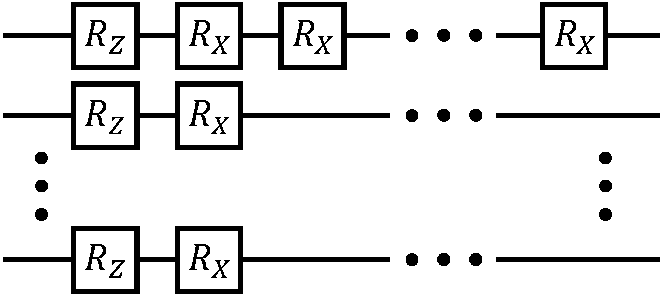
\includegraphics[width=0.9\textwidth]{figures/Z_Ansatz.pdf} \caption{难以多项式时间模拟的线路例子:每个量子比特上有一层 $R_Z$ 门,每个量子比特上有一层 $R_X$ 门,第一个量子比特上有 $L-2$ 层 $R_X$ 门。}\label{ap:prop:fig:ansatz} 
\end{figure}

如果截断含噪声期望值 $\abs{\bm{s}}\leq L$,估计的期望值可以表示为: 
\begin{equation} 
    \widehat{\langle O \rangle}=\sum_{\abs{s}\leq L} f(\widetilde{\mathcal{U}},\bm{s},O,\rho)=\sum_{m=0}^L (1-\lambda)^m \sum_{\abs{s}=m} f(\mathcal{U},\bm{s},O,\rho).
\end{equation}

在考虑 $\widetilde{\langle O \rangle}$ 和 $\widehat{\langle O \rangle}$ 之间的差异之前,我们首先考虑无噪声情况。第一个量子比特上的酉矩阵可以表示为: 
\begin{equation} 
    U|_1=\exp{-i\frac{\theta_{2,1}+\cdots+\theta_{L,1} }{2}X_1}\exp{-i\frac{\theta_{1,1}}{2}Z_1}.
\end{equation} 
记 $\alpha=\frac{\theta_{2,1}+\cdots+\theta_{L,1} }{2}$,无噪声理想期望值可以表示为: 
\begin{equation}\label{ap:eq:noiseless_cost} 
    \begin{aligned} 
        \langle O \rangle&=\bra{0}\exp{-i\frac{\theta_{1,1}}{2}Z_1}^\dagger\exp{-i \alpha X_1}^\dagger (Z_1+Y_1) \exp{-i \alpha X_1}\exp{-i\frac{\theta_{1,1}}{2}Z_1}\ket{0}\\
        &=\cos{2\alpha}-\sin{2\alpha}. 
    \end{aligned} 
\end{equation}

注意在第~\ref{sec:obppp}节中,我们讨论了对于具有非零贡献的 Pauli 路径 $\bm{s}$,必须有 $\abs{s_i} > 0$ 对于 $i=0,\cdots,L$成立。因此需要 $\abs{\bm{s}}\geq L+1$。

相反,若对于某个Pauli路径$\bm{s}$,如果 $\abs{\bm{s}}> L+1$且存在一个量子比特 $k\neq 1$,使得 $s_{i}|_k$ 在某些层 $i$ 上不是单位算符,则因为$O|_k=I$,会有 $f(\mathcal{U},\bm{s},O,\rho)=0$ 成立。
因此,对 $\langle O \rangle(\theta)$ 有非零贡献的 Pauli 路径 $\bm{s}$ 必须满足 $\abs{s}=L+1$。 
我们可以得出结论: 
\begin{equation}\label{ap:eq:noiseless_cost_2} 
    \begin{aligned} \langle O \rangle=\sum_{s\in \bm{P}^{L+1}_n} f(\mathcal{U},\bm{s},O,\rho)=\sum_{\abs{\bm{s}}=L+1} f(\mathcal{U},\bm{s},O,\rho).
    \end{aligned} 
\end{equation}

结合等式~\eqref{ap:eq:noiseless_cost} 和式~\eqref{ap:eq:noiseless_cost_2},可以得到: 
\begin{equation} 
    \mathbb{E}_{\bm{\theta}}\langle O \rangle^2=\mathbb{E}_{\bm{\theta}} \left[\sum_{\abs{s}=L+1} f(\mathcal{U},\bm{s},O,\rho) \right]^2=\mathbb{E}_{\alpha}(\cos{2\alpha}-\sin{2\alpha})^2=\mathbb{E}{\alpha}[1-\sin4\alpha]=1. 
\end{equation} 
上述方程中的最后一个等式是因为 $\alpha$ 遵循广义 Irwin-Hall 分布,其特征函数 $\varphi_{\alpha}(t)=\mathbb{E}[e^{it\alpha}]$ 可以表示为 $\left(\frac{e^{i\frac{\pi}{2}t}-e^{-i\frac{\pi}{2}t}}{i\pi t}\right)^{L-1}$。于是,有 
\begin{equation} 
    \mathbb{E}_{\alpha}[\sin4\alpha]=\textrm{Im }\mathbb{E}[e^{i4\alpha}]=\textrm{Im }\varphi_{\alpha}(4)=\textrm{Im }\left(\frac{e^{2\pi i}-e^{-2\pi i}}{4\pi i}\right)^{L-1}=0.
\end{equation}

综上所述,对于$\widetilde{\langle O \rangle}$ 和 $\widehat{\langle O \rangle}$ 之间的均方误差可以估计为: 
\begin{equation} 
    \begin{aligned} 
        \mathbb{E}_{\bm{\theta}}\abs{\widetilde{\langle O \rangle}-\widehat{\langle O \rangle}}^2 &=\mathbb{E}_{\bm{\theta}}\left[\sum_{\abs{s}> L}f(\widetilde{\mathcal{U}},\bm{s},O,\rho)\right]^2\\
         &=\mathbb{E}_{\bm{\theta}}\left[\sum_{\abs{s}=L+1}f(\widetilde{\mathcal{U}},\bm{s},O,\rho)\right]^2\\
        &= (1-\lambda)^{2(L+1)}\mathbb{E}_{\bm{\theta}} \left[\sum_{\abs{s}=L+1}{f}(\mathcal{U},\bm{s},O,\rho)\right]^2\\ 
        &=(1-\lambda)^{2(L+1)}.
    \end{aligned} 
\end{equation}

根据伯努利不等式,对于 $r\geq 1$ 和 $x\geq -1$,有 
\begin{equation} 
    (1+x)^r\geq 1+r. 
\end{equation}

由于 $\lambda=\order{\frac{1}{L}}$,存在一个常数 $c$ 使得 $c\geq \lambda (L+1)$。因此,我们有 \begin{equation} 
    (1-\lambda)^{2(L+1)}= (1-\lambda)^{\frac{2(L+1)}{4c} 4c} \geq \left(1-\lambda \frac{2(L+1)}{4c} \right)^{4c}\geq \left(\frac{1}{2}\right)^{4c}, 
\end{equation} 
此时有
\begin{equation} 
    \mathbb{E}_{\bm{\theta}}\abs{\widetilde{\langle O \rangle}-\widehat{\langle O \rangle}}^2 =\Omega(1). 
\end{equation}

所以截断 $\abs{s}\leq L$ 是不够的。 而具有非零贡献且满足 $\abs{\bm{s}}=L+1$ 的 Pauli 路径的数量为 $2^{L-1}$,具体为:
\begin{equation} 
    \begin{aligned}
        &\bm{s}=(s_0,s_1,\cdots,s_L)=(Z_1,Z_1,\cdots,Z_1,Y_1),\\
        &s_0=Z_1, \quad s_1=Z_1, \quad s_2=\begin{cases}
            Z_1 \\ \text{或}\\
            Y_1,
        \end{cases}
        \cdots, s_L=\begin{cases}
            Z_1 \\ \text{或} \\
            Y_1.
        \end{cases}
    \end{aligned}
\end{equation}

因此,对于 $\gamma=\order{\frac{1}{L}}$,我们需要考虑所有具有非零贡献的 Pauli 路径,这将导致指数时间成本。这完成了命题~\ref{prop:lambda_and_L}的证明。


\section{本章小结}

本章介绍了变分量子线路的基本结构,以及对含噪声环境下模拟变分量子的意义。并使用基于Pauli路径积分的OBPPP算法实现对含噪声变分量子线路的模拟,并分析了算法的复杂度及对应的模拟误差。最后,我们讨论了在噪声率与线路深度之间的关系下,模拟算法的有效性。

主要结果通过定理~\ref{thm:main}刻画,即对于含有常数噪声的变分量子线路,在满足初始态密度矩阵和观测量都是稀疏以及条件~\ref{eq:generate}成立的情况下,存在多项式量级的经典算法可以在高效近似地模拟含噪声的变分量子线路。这意味着在考虑现有实验条件下,在NISQ设备上运行的变分量子算法很难相对经典算法提供实际的量子优势。

此外,我们还探讨了在未来量子设备的发展中,若要在含噪声的设备上实现量子优势需要满足的必要条件,该结果通过命题~\ref{prop:lambda_and_L}呈现。需要设备的噪声率$\gamma$与线路深度$L$满足$\gamma=o(\frac{1}{\log L})$,才有可能呈现出量子优势。这一结果对于未来量子设备的发展具有一定的指导意义。